\documentclass[lang=cn,12pt,scheme=chinese]{elegantbook}

\title{数学分析(B1)课程讲义}

\bioinfo{简介}{
    本讲义为汪琥庭老师2024秋季学期数学分析B1课程讲义的latex整理版,不包括复习课内容.
}
\date{\today}
\version{2.0}
\author{助教 刘越}

\setcounter{tocdepth}{3}
\cover{cover.jpg}

\extrainfo{\bfseries 本讲义仅供学习交流使用,未经许可请勿用于商业目的.\\
如有错误或疏漏请联系邮箱:\url{liuyue22@ustc.mail.edu.cn}\\
\href{https://passiflora-sago.github.io/24FallMAB1.html}{课程主页} \quad
\href{https://github.com/Passiflora-sago/Passiflora-sago.github.io/releases/download/v1.0.0/maexams_2025-v1.pdf}{往年卷汇总}}


% 本文档命令
\usepackage{array}
\newcommand{\ccr}[1]{\makecell{{\color{#1}\rule{1cm}{1cm}}}}

% 修改标题页的橙色带
\definecolor{customcolor}{RGB}{32,178,170}
\colorlet{coverlinecolor}{customcolor}
\usepackage{cprotect}

\addbibresource[location=local]{reference.bib} % 参考文献,不要删除

%# -*- coding: utf-8 -*-

% preamble_command_mathematics_v1_0.tex

% ---------- macro definition ----------
% ----- equation setting -----
\everymath{\displaystyle}

% ----- command -----
\newcommand{\les}{\leqslant}
\newcommand{\ges}{\geqslant}
\newcommand{\degree}{^{\circ}}
\newcommand{\circA}{\overset{\circ}{\mathrm{A}}}
\newcommand{\dageq}{\stackrel{\dag}{ = }}
\newcommand{\ddageq}{\stackrel{\ddag}{ = }}
\newcommand{\dbdageq}{\stackrel{\dbdag}{ = }}
\newcommand{\stareq}{\stackrel{*}{ = }}
\newcommand{\dagiff}{\stackrel{\dag}{\iff}}
\newcommand{\ddagiff}{\stackrel{\ddag}{\iff}}
\newcommand{\dagimp}{\stackrel{\dag}{\implies}}
\newcommand{\ddagimp}{\stackrel{\ddag}{\implies}}
\newcommand{\tensor}[1]{\overleftrightarrow{#1}}
% \renewcommand\tensor[1]{\overset{\scriptscriptstyle\leftrightarrow}{#1}}
\renewcommand{\tensor}[1]{\overset{\scriptstyle\leftrightarrow}{#1}}
\newcommand{\by}{\leftarrow}

\newcommand{\join}{\Join}

% \renewcommand\pi{\piup}
\newcommand{\PI}{\uppi}
% \renewcommand\pi{\uppi}
% \renewcommand\pi{\text{\textpi}}
% \renewcommand\pi{\textrm{\greektext p}}

\newcommand{\nimplies}{\centernot\implies}
\newcommand{\nimpliedby}{\centernot\impliedby}

\renewcommand{\Re}{\mathrm{Re}\,}
\renewcommand{\Im}{\mathrm{Im}\,}
\newcommand{\const}{\mathrm{Const.}}
\newcommand{\sym}{\mathrm{sym}}
\newcommand{\cyc}{\mathrm{cyc}}
\newcommand{\ii}{\,\mathrm{i}}
\newcommand{\jj}{\,\mathrm{j}}

\DeclareMathOperator{\sgn}{sgn}
\DeclareMathOperator{\dif}{d\!}
\DeclareMathOperator{\diff}{d}
\DeclareMathOperator{\trans}{T}
\DeclareMathOperator{\tr}{tr}
\DeclareMathOperator{\grad}{\mathbf{grad}}
\DeclareMathOperator{\rank}{rank}
\DeclareMathOperator{\diag}{diag}
\DeclareMathOperator{\sinc}{sinc}
\DeclareMathOperator{\ad}{ad}
\DeclareMathOperator{\ex}{E}
\DeclareMathOperator{\var}{Var}
\DeclareMathOperator{\argmin}{arg\,min}
\DeclareMathOperator{\argmax}{arg\,max}
\DeclareMathOperator{\softmax}{softmax}
\DeclareMathOperator{\arccot}{arccot}
\DeclareMathOperator{\st}{s.t.}
\DeclareMathOperator{\iid}{i.i.d.}
\DeclareMathOperator{\Exp}{Exp}
\DeclareMathOperator{\Poi}{Poi}

\renewcommand{\parallel}{/\!\!/}

\newcommand{\bR}{\bm{\mathcal{R}}}

\newcommand{\Alpha}{\mathrm{A}}
\newcommand{\Beta}{\mathrm{B}}
\newcommand{\Epsilon}{\mathrm{E}}

\newcommand{\rA}{\mathrm{A}}
\newcommand{\rB}{\mathrm{B}}
\newcommand{\rC}{\mathrm{C}}
\newcommand{\rD}{\mathrm{D}}
\newcommand{\rE}{\mathrm{E}}
\newcommand{\rF}{\mathrm{F}}
\newcommand{\rG}{\mathrm{G}}
\newcommand{\rH}{\mathrm{H}}
\newcommand{\rI}{\mathrm{I}}
\newcommand{\rJ}{\mathrm{J}}
\newcommand{\rK}{\mathrm{K}}
\newcommand{\rL}{\mathrm{L}}
\newcommand{\rM}{\mathrm{M}}
\newcommand{\rN}{\mathrm{N}}
\newcommand{\rO}{\mathrm{O}}
\newcommand{\rP}{\mathrm{P}}
\newcommand{\rQ}{\mathrm{Q}}
\newcommand{\rR}{\mathrm{R}}
\newcommand{\rS}{\mathrm{S}}
\newcommand{\rT}{\mathrm{T}}
\newcommand{\rU}{\mathrm{U}}
\newcommand{\rV}{\mathrm{V}}
\newcommand{\rW}{\mathrm{W}}
\newcommand{\rX}{\mathrm{X}}
\newcommand{\rY}{\mathrm{Y}}
\newcommand{\rZ}{\mathrm{Z}}
\newcommand{\ra}{\mathrm{a}}
\newcommand{\rb}{\mathrm{b}}
\newcommand{\rc}{\mathrm{c}}
\newcommand{\rd}{\mathrm{d}}
\newcommand{\re}{\mathrm{e}}
\newcommand{\rf}{\mathrm{f}}
\newcommand{\rg}{\mathrm{g}}
\newcommand{\rh}{\mathrm{h}}
\newcommand{\ri}{\mathrm{i}}
\newcommand{\rj}{\mathrm{j}}
\newcommand{\rk}{\mathrm{k}}
\newcommand{\rl}{\mathrm{l}}
\renewcommand{\rm}{\mathrm{m}}
\newcommand{\rn}{\mathrm{n}}
\newcommand{\ro}{\mathrm{o}}
\newcommand{\rp}{\mathrm{p}}
\renewcommand{\rq}{\mathrm{q}}
\newcommand{\rr}{\mathrm{r}}
\newcommand{\rs}{\mathrm{s}}
\newcommand{\rt}{\mathrm{t}}
\newcommand{\ru}{\mathrm{u}}
\newcommand{\rv}{\mathrm{v}}
\newcommand{\rw}{\mathrm{w}}
\newcommand{\rx}{\mathrm{x}}
\newcommand{\ry}{\mathrm{y}}
\newcommand{\rz}{\mathrm{z}}

\newcommand{\0}{\bm{0}}
\newcommand{\1}{\bm{1}}
\newcommand{\A}{\bm{A}}
\newcommand{\B}{\bm{B}}
\newcommand{\C}{\bm{C}}
\newcommand{\D}{\bm{D}}
\newcommand{\E}{\bm{E}}
\newcommand{\F}{\bm{F}}
\newcommand{\G}{\bm{G}}
\renewcommand{\H}{\bm{H}}
\newcommand{\I}{\bm{I}}
\newcommand{\J}{\bm{J}}
\newcommand{\K}{\mathbb{K}}
\renewcommand{\L}{\bm{L}}
\newcommand{\M}{\bm{M}}
\newcommand{\N}{\mathbb{N}}
\renewcommand{\O}{\bm{O}}
\renewcommand{\P}{\bm{P}}
\newcommand{\Q}{\mathbb{Q}}
\newcommand{\R}{\mathbb{R}}
\renewcommand{\S}{\bm{S}}
\newcommand{\T}{\bm{T}}
\newcommand{\U}{\bm{U}}
\newcommand{\V}{\bm{V}}
\newcommand{\W}{\bm{W}}
\newcommand{\X}{\bm{X}}
\newcommand{\Y}{\bm{Y}}
\newcommand{\Z}{\mathbb{Z}}
\renewcommand{\a}{\bm{a}}
\renewcommand{\b}{\bm{b}}
\renewcommand{\c}{\bm{c}}
\renewcommand{\d}{\bm{d}}
\newcommand{\e}{\mathrm{e}}
\newcommand{\f}{\bm{f}}
\newcommand{\g}{\bm{g}}
\newcommand{\h}{\bm{h}}
\renewcommand{\i}{\bm{i}}
\renewcommand{\j}{\bm{j}}
\renewcommand{\k}{\bm{k}}
\renewcommand{\l}{\bm{l}}
\newcommand{\m}{\bm{m}}
\newcommand{\n}{\bm{n}}
\renewcommand{\o}{\bm{o}}
\newcommand{\p}{\bm{p}}
\newcommand{\q}{\bm{q}}
% \renewcommand\r{\bm{r}}
\newcommand{\br}{\bm{r}}
\newcommand{\s}{\bm{s}}
\renewcommand{\t}{\bm{t}}
\renewcommand{\u}{\bm{u}}
\renewcommand{\v}{\bm{v}}
\newcommand{\w}{\bm{w}}
\newcommand{\x}{\bm{x}}
\newcommand{\y}{\bm{y}}
\newcommand{\z}{\bm{z}}

\newcommand{\balpha}{\bm{\alpha}}
\newcommand{\bbeta}{\bm{\beta}}
\newcommand{\bchi}{\bm{\chi}}
\newcommand{\bdelta}{\bm{\delta}}
\newcommand{\bvarepsilon}{\bm{\varepsilon}}
\newcommand{\bphi}{\bm{\phi}}
\newcommand{\bvarphi}{\bm{\varphi}}
\newcommand{\bgamma}{\bm{\gamma}}
\newcommand{\bmeta}{\bm{\eta}}
\newcommand{\biota}{\bm{\iota}}
\newcommand{\bkappa}{\bm{\kappa}}
\newcommand{\blambda}{\bm{\lambda}}
\newcommand{\bvarLambda}{\bm{\varLambda}}
\newcommand{\bmu}{\bm{\mu}}
\newcommand{\bnu}{\bm{\nu}}
\newcommand{\bpi}{\bm{\pi}}
\newcommand{\bvarpi}{\bm{\varpi}}
\newcommand{\btheta}{\bm{\theta}}
\newcommand{\bvartheta}{\bm{\vartheta}}
\newcommand{\brho}{\bm{\rho}}
\newcommand{\bsigma}{\bm{\sigma}}
\newcommand{\bvarsigma}{\bm{\varsigma}}
\newcommand{\btau}{\bm{\tau}}
\newcommand{\bupsilon}{\bm{\upsilon}}
\newcommand{\bomega}{\bm{\omega}}
\newcommand{\bxi}{\bm{\xi}}
\newcommand{\bpsi}{\bm{\psi}}
\newcommand{\bzeta}{\bm{\zeta}}
\newcommand{\bAlpha}{\bm{\Alpha}}
\newcommand{\bBeta}{\bm{\Beta}}
\newcommand{\bChi}{\bm{\Chi}}
\newcommand{\bDelta}{\bm{\Delta}}
\newcommand{\bEpsilon}{\bm{\Epsilon}}
\newcommand{\bPhi}{\bm{\Phi}}
\newcommand{\bGamma}{\bm{\Gamma}}
\newcommand{\bEta}{\bm{\Eta}}
\newcommand{\bIota}{\bm{\Iota}}
\newcommand{\bKappa}{\bm{\Kappa}}
\newcommand{\bLambda}{\bm{\Lambda}}
\newcommand{\bMu}{\bm{\Mu}}
\newcommand{\bNu}{\bm{\Nu}}
\newcommand{\bPi}{\bm{\Pi}}
\newcommand{\bTheta}{\bm{\Theta}}
\newcommand{\bRho}{\bm{\Rho}}
\newcommand{\bSigma}{\bm{\Sigma}}
\newcommand{\bvarSigma}{\bm{\varSigma}}
\newcommand{\bTau}{\bm{\Tau}}
\newcommand{\bUpsilon}{\bm{\Upsilon}}
\newcommand{\bOmega}{\bm{\Omega}}
\newcommand{\bXi}{\bm{\Xi}}
\newcommand{\bPsi}{\bm{\Psi}}
\newcommand{\bZeta}{\bm{\Zeta}}
\newcommand{\ve}{\varepsilon}
\newcommand{\laplace}{\Delta}

% 启用 expl3 语法处理多个变量
\ExplSyntaxOn

% 定义 \parfrac 宏,默认阶数为 1,支持多个变量
\NewDocumentCommand{\parfrac}{O{1} m m}
{
  \frac{
    \int_compare:nNnTF {#1} = {1} {\partial #2} {\partial^{#1} #2}
  }
  {
    \parfrac_process_vars:n { #3 }
  }
}

% 处理逗号分隔的多个偏导变量
\cs_new_protected:Nn \parfrac_process_vars:n
{
  \seq_set_split:Nnn \l_tmpa_seq { , } { #1 }
  \seq_map_inline:Nn \l_tmpa_seq { \partial ##1 }
}

\ExplSyntaxOff

\definecolor{structurecolor}{RGB}{60,113,183}
\definecolor{main}{RGB}{76,141,174}
\definecolor{second}{RGB}{213,180,92}
\definecolor{third}{RGB}{120,146,98}




\begin{document}
%设置章节计数器为2
\setcounter{chapter}{4}
\setcounter{chapter}{4}
\chapter{空间解析几何综述}'

\section{坐标系的平移与旋转}

\begin{example}
    设有二次曲面$\Sigma:4x^2+25y^2+4z^2-16x-50y-16z-4z=0$,

    \begin{enumerate}
        \item 指出$\Sigma$是何种二次曲面;
        \item 将$\Sigma$一般化为参数式.
    \end{enumerate}
\end{example}\

\begin{solution}
\begin{enumerate}
    \item 配方得,$4(x-2)^2+25(y-1)^2+4(z-2)^2 = 100$,即
    $$
    \frac{(x-2)^2}{5^2}+\frac{(y-1)^2}{2^2}+\frac{(z-2)^2}{5^2} = 1
    $$
    故$\Sigma$是一个旋转椭球面.

    若令$\begin{cases}
        x-2 = x'\\
        y-1 = y'\\
        z-2 = z'
    \end{cases},M_0 = (2,1,2)=O'$,即是将坐标系的原点平移到$M_0$点,记作$O'$,新的经过平行移动得到的坐标系为$O'-x'y'z'$.
    在新坐标系下,$\Sigma$的方程为
    $$
    \frac{x'^2}{5^2}+\frac{y'^2}{2^2}+\frac{z'^2}{5^2} = 1
    $$
    \item 若令$\begin{cases}
        \frac{x'}{5} = \sin \theta \cos \varphi\\
        \frac{y'}{2} = \sin \theta \sin \varphi\\
        \frac{z'}{5} = \cos \theta
    \end{cases}$,则$\begin{cases}
        x' = 5\sin \theta \cos \varphi\\
        y' = 2\sin \theta \sin \varphi\\
        z' = 5\cos \theta
    \end{cases}, \theta \in [0,\pi],\varphi \in [0,2\pi]$
    即$\Sigma$的参数方程为
    $$
    \begin{cases}
        x = 2 + 5 \sin \theta \cos \varphi\\
        y = 1 + 2 \sin \theta \sin \varphi\\
        z = 2 + 5 \cos \theta
    \end{cases}, \theta \in [0,\pi],\varphi \in [0,2\pi]
    $$
    其中$\begin{cases}
        x' = 5\sin \theta \cos \varphi\\
        y' = 2\sin \theta \sin \varphi\\
        z' = 5\cos \theta
    \end{cases}, \theta \in [0,\pi],\varphi \in [0,2\pi]$是在新坐标系下的参数式,
    $\begin{cases}
        x = 2 + 5 \sin \theta \cos \varphi\\
        y = 1 + 2 \sin \theta \sin \varphi\\
        z = 2 + 5 \cos \theta
    \end{cases}, \theta \in [0,\pi],\varphi \in [0,2\pi]$是在原坐标系下的参数式.
\end{enumerate}
\end{solution}

\begin{remark}
    曲面$\Sigma$的参数式都是双参数的,但是参数式不是唯一的,例如
    $$
    \begin{cases}
        x = 2 + 5 \cos \theta \cos \varphi\\
        y = 1 + 2 \cos \theta \sin \varphi\\
        z = 2 + 5 \sin \theta
    \end{cases}, \theta \in [-\frac{\pi}{2},\frac{\pi}{2}],\varphi \in [0,2\pi]
    $$
    也是$\Sigma$的参数式.
\end{remark}

\begin{example}
    设有二次曲面$\Sigma:xy=z.$
    \begin{enumerate}
        \item 指出$\Sigma$是何种二次曲面;
        \item 求$\Sigma$的参数式.
    \end{enumerate}
\end{example}

\begin{solution}
    若保持坐标系的原点不动,让坐标系进行旋转变化.设$O-xyz$坐标系中,基向量为$\i,\j,\k$,在$O-x'y'z'$坐标系中,基向量为$\i',\j',\k'$,且$\i',\j',\k'$与$\i,\j,\k$的夹角如下表所示:
    \begin{table}[htbp]\label{ijk-i'j'k'}
        \centering
        \begin{tabular}{|c|c|c|c|}
            \hline
            & $\i$ & $\j$ & $\k$\\
            \hline
            $\i'$ & $\alpha_1$ & $\beta_1$ & $\gamma_1$\\
            \hline
            $\j'$ & $\alpha_2$ & $\beta_2$ & $\gamma_2$\\
            \hline
            $\k'$ & $\alpha_3$ & $\beta_3$ & $\gamma_3$\\
            \hline
        \end{tabular}
        \caption{}
    \end{table}

    \begin{figure}[htbp]
        \centering
        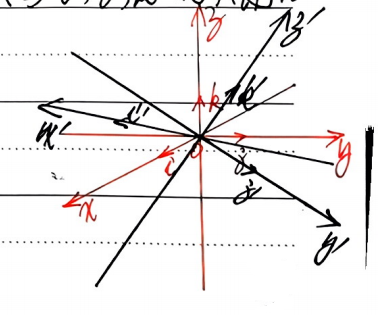
\includegraphics[width=0.3\textwidth]{figure/5-1.png}
        \caption{}
    \end{figure}

设$\overrightarrow{OM} = (a,b,c) \neq \theta$,则$\overrightarrow{OM}^\circ = \frac{\overrightarrow{OM}}{|\overrightarrow{OM}|} = (\frac{a}{|\overrightarrow{OM}|},\frac{b}{|\overrightarrow{OM}|},\frac{c}{|\overrightarrow{OM}|}) = (\cos \alpha, \cos \beta, \cos \gamma) = \cos \i + \cos \j + \cos \k$.
即单位向量$\overrightarrow{OM}^\circ$可以用他的三个方向余弦作为坐标,由表5.1得
$$
\begin{cases}
    \i' = \cos \alpha_1 \i + \cos \beta_1 \j + \cos \gamma_1 \k\\
    \j' = \cos \alpha_2 \i + \cos \beta_2 \j + \cos \gamma_2 \k\\
    \k' = \cos \alpha_3 \i + \cos \beta_3 \j + \cos \gamma_3 \k
\end{cases}
$$

现设点$Q$在$O-xyz$坐标系的坐标为$Q(x,y,z)$,在$O-x'y'z'$坐标系的坐标为$Q'(x',y',z')$,则
\begin{align*}
    \overrightarrow{OQ} &= x\i + y\j + z\k = x'\i' + y'\j' + z'\k'\\
    &= x'(\cos \alpha_1 \i + \cos \beta_1 \j + \cos \gamma_1 \k) + y'(\cos \alpha_2 \i + \cos \beta_2 \j + \cos \gamma_2 \k) + z'(\cos \alpha_3 \i + \cos \beta_3 \j + \cos \gamma_3 \k)\\
    &= (x' \cos \alpha_1 + y' \cos \alpha_2 + z' \cos \alpha_3)\i + (x' \cos \beta_1 + y' \cos \beta_2 + z' \cos \beta_3)\j + (x' \cos \gamma_1 + y' \cos \gamma_2 + z' \cos \gamma_3)\k
\end{align*}

也就是得到了
$$
\begin{cases}\label{X=AX'}
    x = x' \cos \alpha_1 + y' \cos \alpha_2 + z' \cos alpha_3\\
    y = x' \cos \beta_1 + y' \cos \beta_2 + z' \cos \beta_3\\
    z = x' \cos \gamma_1 + y' \cos \gamma_2 + z' \cos \gamma_3
\end{cases}
$$

若令$\X = \begin{pmatrix}
    x\\
    y\\
    z   
\end{pmatrix} , A = \begin{pmatrix}
    \cos \alpha_1 & \cos \alpha_2 & \cos \alpha_3\\
    \cos \beta_1 & \cos \beta_2 & \cos \beta_3\\
    \cos \gamma_1 & \cos \gamma_2 & \cos \gamma_3
\end{pmatrix} , \X' = \begin{pmatrix}
    x'\\
    y'\\
    z'
\end{pmatrix}$,则有$\X = A\X'$,即$\X' = A^{-1}\X$,其中$A$的各行各列都是单位向量,且任意两行(列)正交;
在线性代数中,称$A$这样的矩阵为正交矩阵,即$AA^T  = A^T A = I$,其中$I$是单位矩阵.
称$\ref{X=AX'}$为正交线性变化,简称正交变换.

不难验证,$A A^T = A^T A = I$,即便几何中的旋转或物理中刚体的旋转,在代数中对应正交变换.\ref{X=AX'}表明旋转之后,原坐标$x,y,z$与新坐标$x',y',z'$之间的对应关系是正交变换关系.

\begin{enumerate}
    \item 若保持$Oz$轴不便,让$Oxy$坐标平面绕$z$轴逆时针旋转$\frac{\pi}{4}$,得到了新坐标系$O-x'y'z'$,则有

\begin{table}[htbp]
    \centering
    \begin{tabular}{|c|c|c|c|}
        \hline
        & $\i$ & $\j$ & $\k$\\
        \hline
        $\i'$ & $\pi / 4$ & $\pi / 4$ & $\pi /2$\\
        \hline
        $\j'$ & $3\pi / 4$ & $\pi / 4$ & $\pi /2$\\
        \hline
        $\k'$ & $\pi / 2$ & $\pi / 2$ & $0$\\
        \hline
    \end{tabular}
\end{table}

即有
$$
\begin{cases}
    x = x' \cos \frac{\pi}{4} + y' \cos \frac{3\pi}{4} + z' \cos \frac{\pi}{2} = \frac{1}{\sqrt{2}}(x'-y')\\
    y = x' \cos \frac{\pi}{4} + y' \cos \frac{\pi}{4} + z' \cos \frac{\pi}{2} = \frac{1}{\sqrt{2}}(x'+y')\\
    z = x' \cos \frac{\pi}{2} + y' \cos \frac{\pi}{2} + z' \cos 0 = z'
\end{cases}
$$

利用此正交变换,可以将$\Sigma:xy=z$化为$\Sigma: \frac{1}{\sqrt{2}}(x'-y')\frac{1}{\sqrt{2}}(x'+y')=z'$,即$z' = \frac{x'^2}{2} - \frac{y'^2}{2}$,即$\Sigma$是一个双曲抛物面.
\item $\Sigma:xy = z$在原坐标系中的参数式为$\begin{cases}
    x = x+0y\\
    y = 0x+y\\
    z = xy
\end{cases}$,$x,y$为参数,则$\Sigma$在新坐标系中的参数式为:$\begin{cases}
    x' = x' +0y'\\
    y' = 0x'+y'\\
    z' = \frac{1}{2}(x'^2-y'^2)
\end{cases}$,$x',y'$为参数.

\end{enumerate}
\end{solution}

\section{柱面坐标系与球面坐标系}

\subsection{柱面坐标系}

$\R^3$空间中任一点$Q(x,y,z)$都可以看作是在半径为$r$的某个圆柱面:$x^2+y^2 = r^2$上.而圆柱面$x^2+y^2=r^2$上的点都可以用$r,\theta,z$这三个参数来确定,称$(r,\theta,z)$为点$Q$的柱面坐标.

\begin{figure}[htbp]
    \centering
    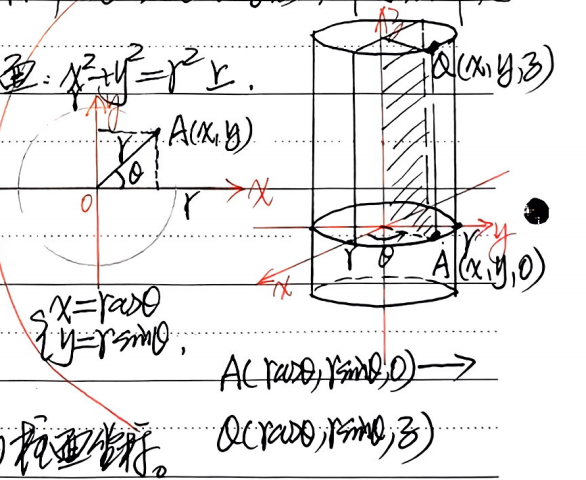
\includegraphics[width=0.3\textwidth]{figure/5-2.png}
    \caption{}
\end{figure}

\subsection{球面坐标系}

$\R^3$空间中任一点$Q(x,y,z)$都位于某个半径为$r$的球面$x^2+y^2+z^2=r^2$上,其中$r = | \overrightarrow{OQ} |$,$\overrightarrow{OQ}$与$Oz$轴的正向的夹角设为$\theta$,$\overrightarrow{OQ}$在$Oxy$平面中的投影与$Ox$轴正向夹角为$\varphi$,$0 \les \theta \les \pi, 0 \les \varphi \les 2 \pi$.
则$y = | \overrightarrow{OA}| \sin \varphi = r \sin \theta \sin \varphi$,而$z = r \cos \theta$.

称$(r,\theta,\varphi)$为点$Q$的球面坐标.球面坐标$r,\theta,\varphi$与直角坐标$x,y,z$之间的关系为
$$
\begin{cases}
    x = r \sin \theta \cos \varphi\\
    y = r \sin \theta \sin \varphi\\
    z = r \cos \theta
\end{cases},\theta \in [0,\pi],\varphi \in [0,2\pi], r \ges 0
$$

\begin{figure}[htbp]
    \centering
    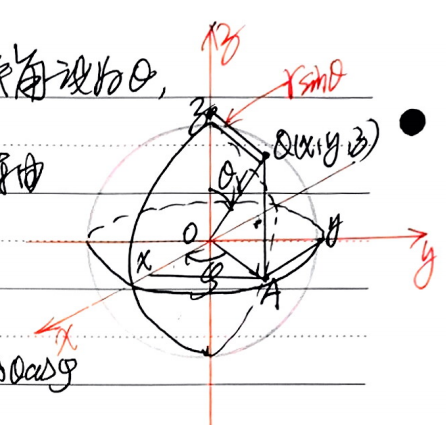
\includegraphics[width=0.3\textwidth]{figure/5-3.png}
    \caption{}
\end{figure}

直角坐标系下的球面方程:$\Sigma:x^2+y^2+z^2 = R^2$在柱面坐标系下$\begin{cases}
    x = r \cos \theta\\
    y = r \sin \theta\\
    z = z
\end{cases}$ 化为$\Sigma:r^2+z^2 = R^2$,即$\Sigma:r = R$.

在球面坐标系中,$\begin{cases}
    x = r \sin \theta \cos \varphi\\
    y = r \sin \theta \sin \varphi\\
    z = r \cos \theta
\end{cases}$下,化为$x^2+y^2+z^2 = r^2 = R^2$,即$\Sigma:r = R$.

双叶双曲面$\Sigma:x^2-y^2-z^2 = 1$在柱面坐标系中化为$r^2 \cos 2 \theta - z^2 = 1$,在球面坐标系中化为$2x^2 - (x^2 + y^2 + z^2) = 2(r \sin \theta \cos \varphi)^2 - r^2 = r^2 ( 2 \sin^2 \theta \cos^2 \varphi -1) = 1$.

\section{空间曲线的参数式}

空间曲线可以写为交线方程组$\begin{cases}
    F(x,y,z) = 0\\
    G(x,y,z) = 0
\end{cases}$,他可以改写为参数式.

\begin{example}
    将空间$\R^3$中的大圆周$\Gamma:\begin{cases}
        x^2+y^2+z^2 = a^2,a >0\\
        x+y+z = 0
    \end{cases}$化为参数式.
\end{example}

\begin{figure}[htbp]
    \centering
    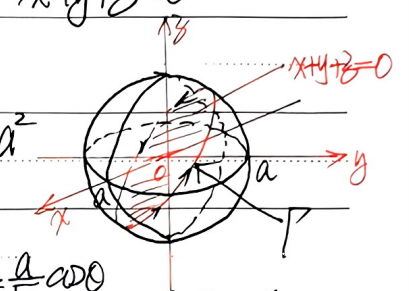
\includegraphics[width=0.3\textwidth]{figure/5-4.png}
    \caption{}
\end{figure}

\begin{solution}
    从$z = -(x+y) \Rightarrow x^2 + y^2 + (x+y)^2 = a^2 \Rightarrow x^2 +xy +y^2 = \frac{a^2}2 \Rightarrow \left( x+ \frac{y}{2} \right)^2 + \left( \frac{\sqrt{3}}{2}y \right)^2 = \left( \frac{a}{\sqrt{2}} \right)^2$.
    令$\begin{cases}
        x + \frac{y}{2} = \frac{a}{\sqrt{2}} \cos \theta\\
        \frac{\sqrt{3}}{2}y = \frac{a}{\sqrt{2}} \sin \theta
    \end{cases}, \theta \in [0,2\pi]$.则$y = \frac{2}{\sqrt{6}} a \sin \theta \Rightarrow x = \frac{a}{\sqrt{6}} (\sqrt3 \cos \theta - \sin \theta) \Rightarrow z = -(x+y) = \frac{-a}{\sqrt 6}(\sqrt 3 \cos \theta + \sin \theta)$.
    即圆周$\Gamma$的参数式为$\begin{cases}
        x = \frac{a}{\sqrt{6}} (\sqrt 3 \cos \theta - \sin \theta)\\
        y = \frac{2}{\sqrt{6}} a \sin \theta\\
        z = \frac{-a}{\sqrt{6}} (\sqrt 3 \cos \theta + \sin \theta)
    \end{cases}, \theta \in [0,2\pi]$.

\end{solution}


    若将$x$视为参数,则从$\begin{cases}
        F(x,y,z) = 0\\
        G(x,y,z) = 0
    \end{cases}$中可以解出$\begin{cases}
        x = x\\
        y = y(x)\\
        z = z(x)
    \end{cases},x \in I$.

\begin{example}
    空间中的直线$\Gamma:\begin{cases}
        x +y+z+5 =0\\
        x-y-2z -1=0
    \end{cases} \Leftrightarrow \begin{cases}
        y+3 = -x-5\\
        -y-2z = -x+1
    \end{cases} \Rightarrow \begin{cases}
        x = x\\
        y = -3x - 9\\
        z = 2x +4
    \end{cases}$.
\end{example}

\begin{remark}
    空间的曲线$\Gamma$的参数式中只有一个参数,且$\Gamma$的参数式不是唯一的.

\end{remark}

\begin{example}
    $\Gamma:\begin{cases}
        x = a \cos \theta\\
        y = a \sin \theta\\
        z = b \theta
    \end{cases},\theta \in [0,+\theta),a,b > 0$所表示的空间光滑曲线,称之为螺旋线.并称$k = 2\pi b$为一个螺距.

    \begin{figure}[htbp]
        \centering
        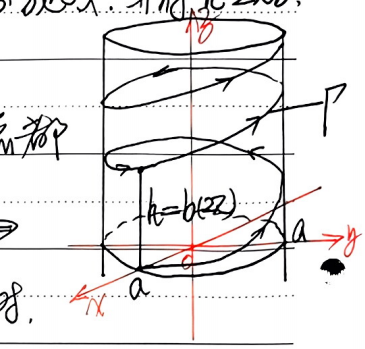
\includegraphics[width=0.3\textwidth]{figure/5-5.png}
        \caption{}
    \end{figure}

    此题中$x^2+y^2 \equiv a^2$,因此$\Gamma$上的点都在圆柱面$x^2+y^2 = a^2$上,而从$z = b \theta \Rightarrow z_\theta ' \equiv b$,即质点在作圆周运动的同时如果向上作匀速运动,
    则综合的结果是沿螺旋线作运动.

    无论是在物理中,还是在几何中,参数增加的方向被认为是曲线$\Gamma$的正向,相反的方向是曲线的负向.
\end{example}

\begin{homework}
ex8.4:1,2,4(4)(5)(6)(10),8,9,11.
\end{homework}


























\end{document}